\documentclass[12pt, oneside]{article}   	% use "amsart" instead of "article" for AMSLaTeX format
\usepackage[margin=1in]{geometry}               % See geometry.pdf to learn the layout options. There are lots.
\geometry{letterpaper}                   	% ... or a4paper or a5paper or ... 
%\geometry{landscape}                		% Activate for rotated page geometry
%\usepackage[parfill]{parskip}    		% Activate to begin paragraphs with an empty line rather than an indent
\usepackage{graphicx}				% Use pdf, png, jpg, or eps§ with pdflatex; use eps in DVI mode
					        % TeX will automatically convert eps --> pdf in pdflatex		

\usepackage[margin=15pt,font={footnotesize,singlespacing},labelfont=bf,labelsep=quad]{caption}
\usepackage{amssymb}
\usepackage{lineno}
% \linenumbers

% Hyperlink
\usepackage{hyperref}
\usepackage{cleveref}[2011/03/22]

%SetFonts
\usepackage[colorinlistoftodos]{todonotes}

\title{\bf{Pandora-based Shower Reconstruction and $\pi^0$ Mass Reconstruction}}
\author{Yun-Tse Tsai}
\date{\today}

\begin{document}
\maketitle

% Introduction
\section{Introduction}


% Shower reconstruction
\section{Shower Reconstruction}

In this section we describe the underlying concepts for shower reconstruction.
The technical details are dispicted in DocDB ?.

% -----------------------------------------------------------------------
\subsection{Brief Introduction to Pandora}

Pandora is a toolkit for pattern recognition, aiming to 
reconstruct particle flow in detectors with fine granularity, such as
detectors of high-energy lepton colliders, and LAr TPC.
MicroBooNE uses Pandora, which is integrated into the LArSoft toolkit
via the \texttt{larpandora} interface,
as one of the pattern recognition and clustering algorithms. \\
\\
% Concept of PFParticle
The outputs of Pandora are centralized in particle-flow particles, 
or PFParticles, which include,
\begin{itemize}
\item PDG code: mainly four types, 11 (shower-like),
      13 (track-like), 12 (neutrino-like PFParticle with a shower-like
      daughter), and 14 (neutrino-like PFParticle with a track-like daughter).
\item Parent: indicates the parent of the PFParticle.
\item Daughters: indicates the daughters (possibly a plural number) of
      the PFParticle.
\end{itemize}
Further, the PFParticles associate to the following objects created
by Pandora,
\begin{itemize}
\item Cluster: collection of hits from a separate hit finding algorithm.
\item Spacepoint: three-dimensional points indicating the 3D positions
      of charge deposition; associating to the two-dimensional hits
      reconstructed by the hit finder.
\item Vertex: a 3D point representing the starting point of the PFParticle.
\item Seed: not generated in a shower-like PFParticle
\item Track
\end{itemize}

In the following sections, we describe the algorithms of shower reconstruction 
utilizing these features.

% -----------------------------------------------------------------------
\subsection{Direction}

An important variable from shower reconstruction is the direction of the 
original electromagnetic particle.
We assume the direction of the vectorial summation of all showering particles 
would retain that of the original particle.
To obtain the direction,
we simply perform a 3-D principal component 
analysis (PCA) over all the spacepoint associated to a PFParticle.
The eigenvector corresponding to the largest eigenvalue determined by
PCA is taken to be the direction of the shower, as it represents the axis
with the largest possible variance of the distribution of the spacepoints.
The forward or backward direction is determined from the ordering of
the spacepoints, which is reconstructed based on the particle flow approach in
the Pandora toolkit.
Further, it will be revisited in the succeeding
shower reconstruction algorithms.\\
\\
In addtion, the (unweighted) 3D centroid of a PFParticle is evaluated
by PCA, and is saved for possible exploitation in other algorithms.

% -----------------------------------------------------------------------
\subsection{Geometry}

% Length, width
The length and the 2D width of a shower is also determined by the same PCA. 

% Opening angle

% -----------------------------------------------------------------------
\subsection{Starting Point}

% -----------------------------------------------------------------------
\subsection{Calorimetry}



% Merging

% MC studies
\section{Simulation Studies}
\label{sec:mc}

In this section, we introduce several shower quality variables to estimate
the quality of shower reconstruction in~\Cref{sec:shr_quality}, and examine
shower reconstruction with simulated single particle Monte Carlo samples
in~\Cref{sec:single_em,sec:single_pi0}.

% -----------------------------------------------------------------------
\subsection{Shower Quality}
\label{sec:shr_quality}

We make plots of variables of reconstructed shower profile, and compare
some of them with simulation.
The object MC shower, which describes the truth level of detectable shower
profile, or the best reconstructed quality that could be achieved, 
is used as the reference point of the comparison.
The details about MC shower can be found in~\cite{DocDB3771}.
Specifically, the direction of MC showers typically represents the truth 
direction of the original electromagnetic particle, while the energy of
MC shower accounts for that deposited in the detector.\\
\\
The shower quality variables are listed below,
\begin{itemize}
\item 3D angle difference, the angular difference in the shower direction 
      between
      MC and reconstructed showers in 3D.
\item Shower length, the length of reconstructed showers, as described
      in~\Cref{sec:shr_geometry}.
\item Starting point difference, the 3D distance between the shower
      starting point of MC shower and that of the reconstructed shower.
\item Clustering efficiency, the ratio of sum of the charges
      in a reconstructed shower to the total deposited charges in
      each wire plane.
\item Energy resolution, $\frac{\textrm{MC deposited energy}-\textrm{Reconstructed energy}}{\textrm{MC deposited energy}}$ in each wire plane.
\item Energy asymmetry, $\frac{\textrm{MC deposited energy}-\textrm{Reconstructed energy}}{\textrm{MC deposited energy}+\textrm{Reconstructed energy}}$ in each wire plane.
\item Energy correlation, a 2D histogram of reconstructed energy versus 
      the MC deposited energy in each wire plane.
\item dQ/dx, dE/dx, the quantities from shower reconstruction.
\item Number of MC (reconstructed) showers, the number of MC (reconstructed)
      showers in each event.
\end{itemize}

% -----------------------------------------------------------------------
\subsection{Single Electromagnetic Particle Sample}
\label{sec:single_em}

We start estimating shower reconstruction qualities with 10,000 simulated
single electron events.
To disentangle different sources of inefficiency, we also prepare a sample
without the bad wires; 
i.e. all the wires in the simulation are good.
The momentum and angle distributions are generated according to
the Laudau distribution,
\begin{equation}
\label{eq:bnb-like}
P(x) = \frac{1}{2\pi i}\int^{c+i\infty}_{c-i\infty}e^{xs+s\log s}ds,
\end{equation}
where, for the momentum distribution, $x = (p-0.3)/0.1$, and $p$ 
represents the modular momentum within a range of 0.1 to 1~GeV.
Similarly, the angular distribution is profiled by setting 
$x = (\theta-0.5)/0.2$,
where $\theta$ is the angle with respect to the $z$-axis ranging from
0 to $2\pi$. \\
\\
We use \texttt{larsoft} and \texttt{uboonecode} \texttt{v05\_08\_00} to
generate the simulated MC samples.
The reconstruction chain is identical to the configuration used in 
the official Monte Carlo challenge~7 (MCC~7), while the simulation 
might have included minor updates.
Nonetheless, there is no significant changes in simulation
since MCC~7.
The MC samples are subsequently larlited with \texttt{larlite} 
\texttt{v05\_02\_00}, and the shower reconstruction is performed in the
\texttt{larlite} framework.\\
\\
% Shower reconstruction
Only the shower-like PFParticles (with a PDG code 11) are selected
as shower candidates and reconstructed in this section.
We extend the selection, and the study is presented 
in~\Cref{sec:merging}. \\
\\
% Results
\Cref{fig:shr_quality_single_em} shows good resolution on 
shower directions and shower starting points.
% In particular, the two variables are better reconstructed in
% electron events, possibly owing to the fact that photons are
% not detected before their pair production.\\
In particular, the quantities are comparative in both the electron
and photon samples, possibly owing to some quality cuts within
the Pandora toolkit.\\
\\
% --------------------------------------------------------------------
% Figure: Shower quality for single e/gamma events
\begin{figure}[htbp]
\begin{center}
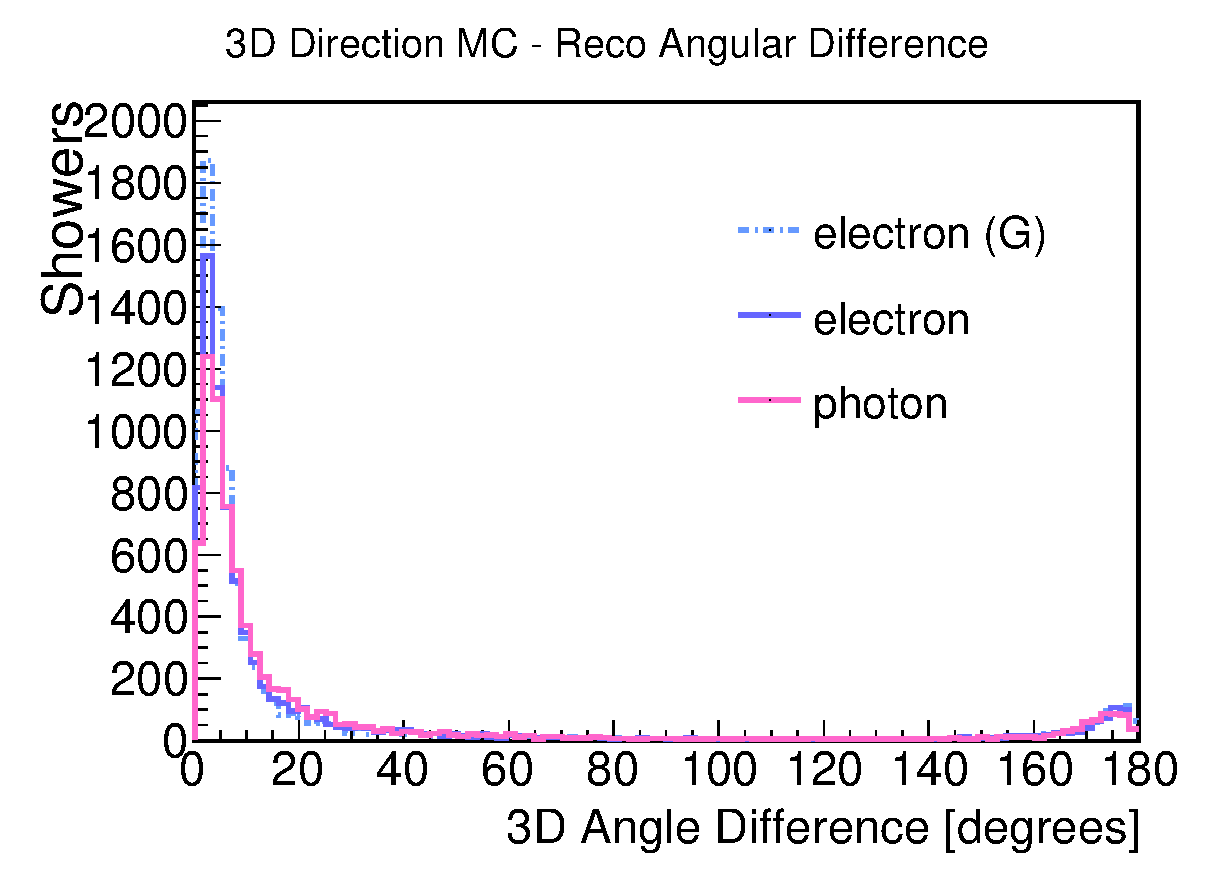
\includegraphics[width=0.3\textwidth]{figs/mc/single_em/AngleDiff.eps}
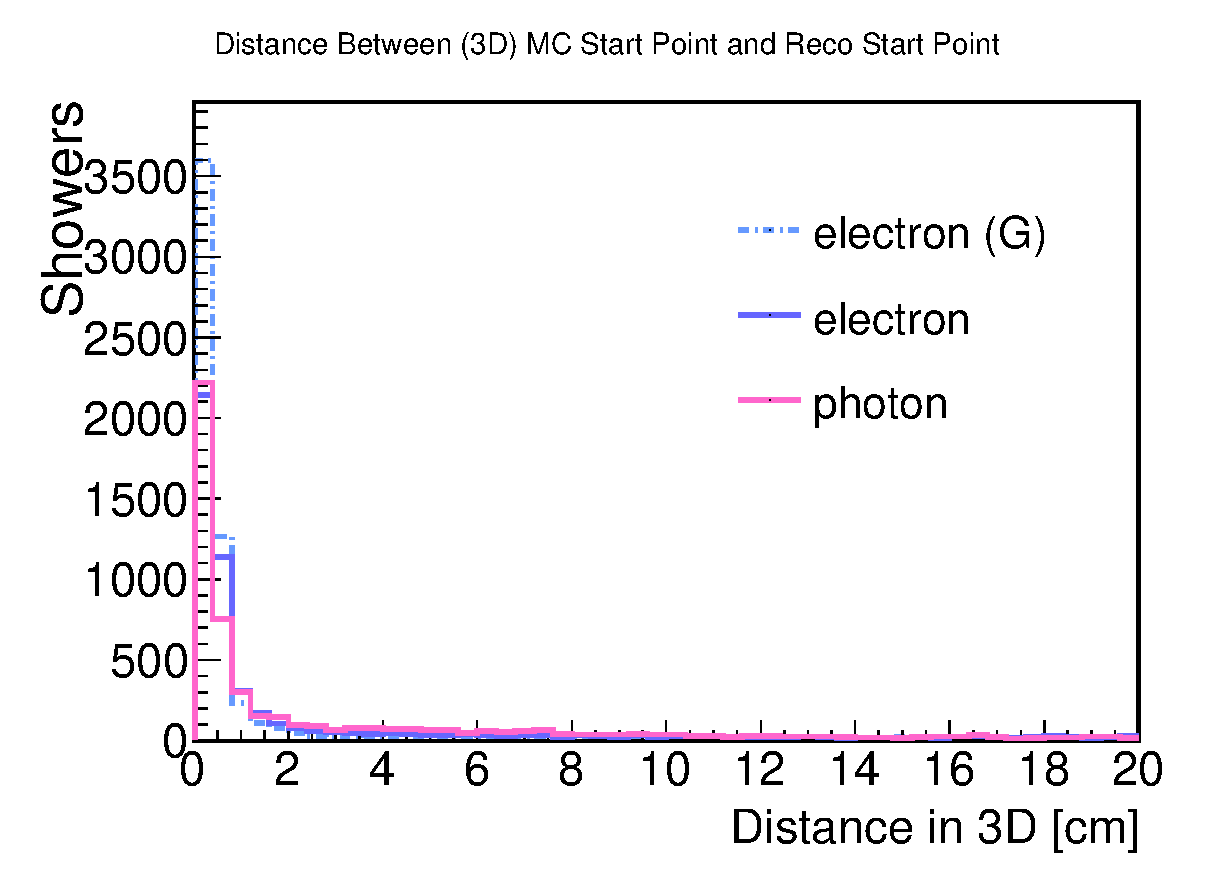
\includegraphics[width=0.3\textwidth]{figs/mc/single_em/StartingPointAcc.eps}
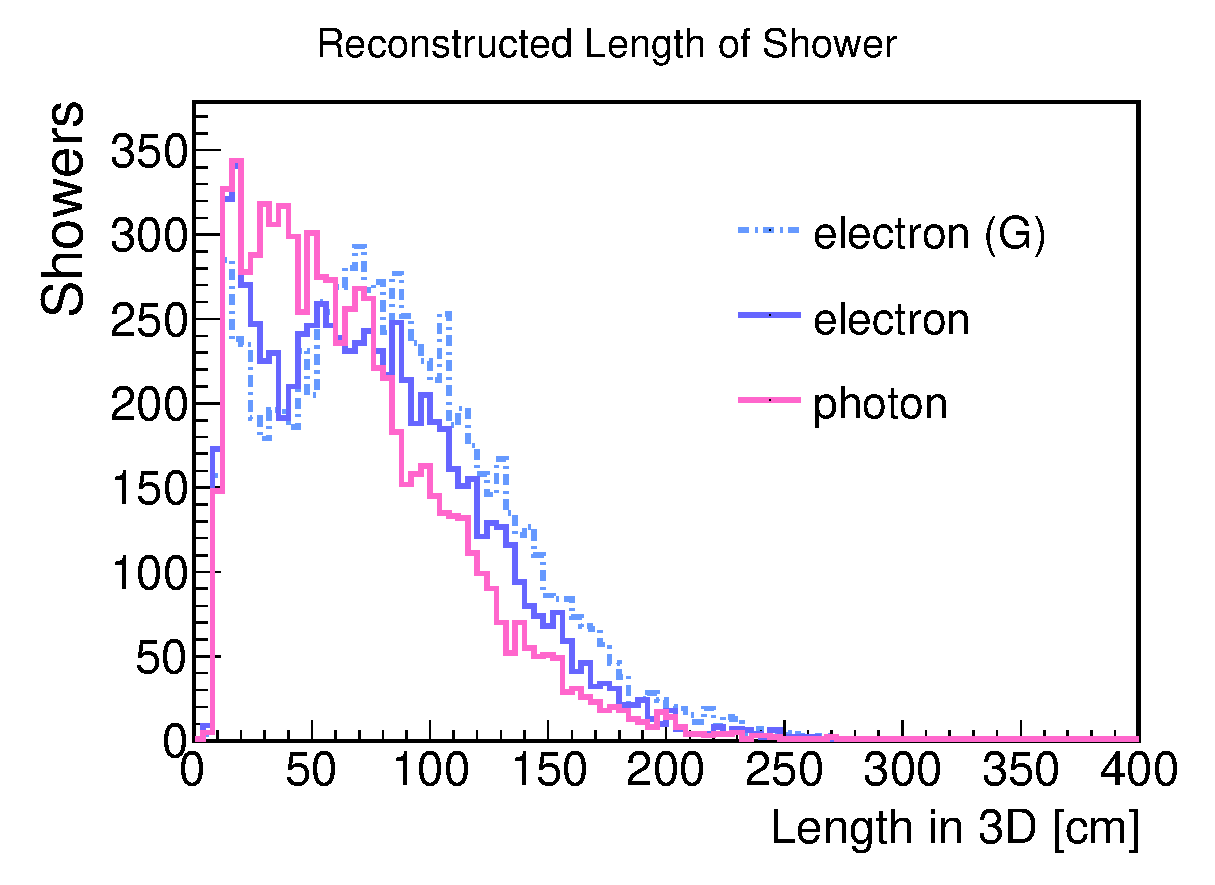
\includegraphics[width=0.3\textwidth]{figs/mc/single_em/Length.eps}
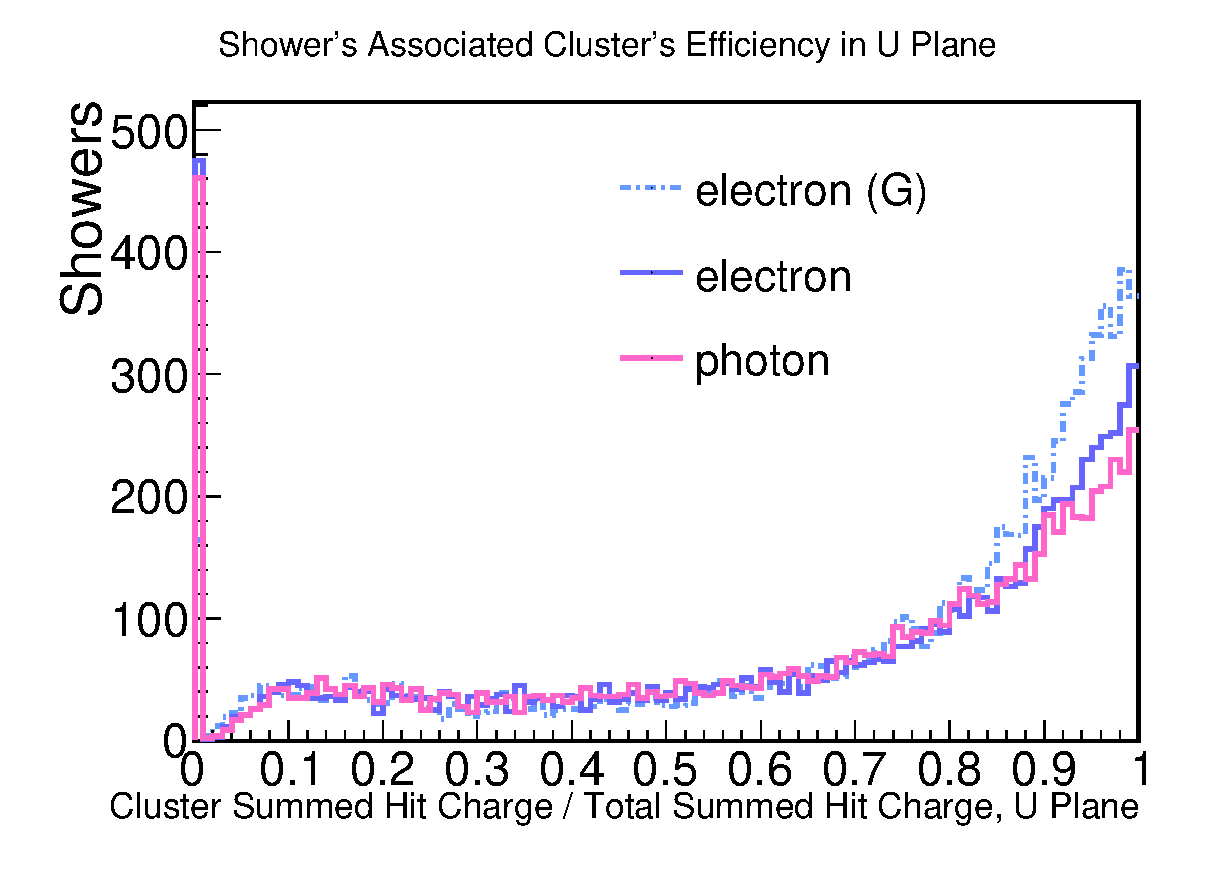
\includegraphics[width=0.3\textwidth]{figs/mc/single_em/ClusterEffU.eps}
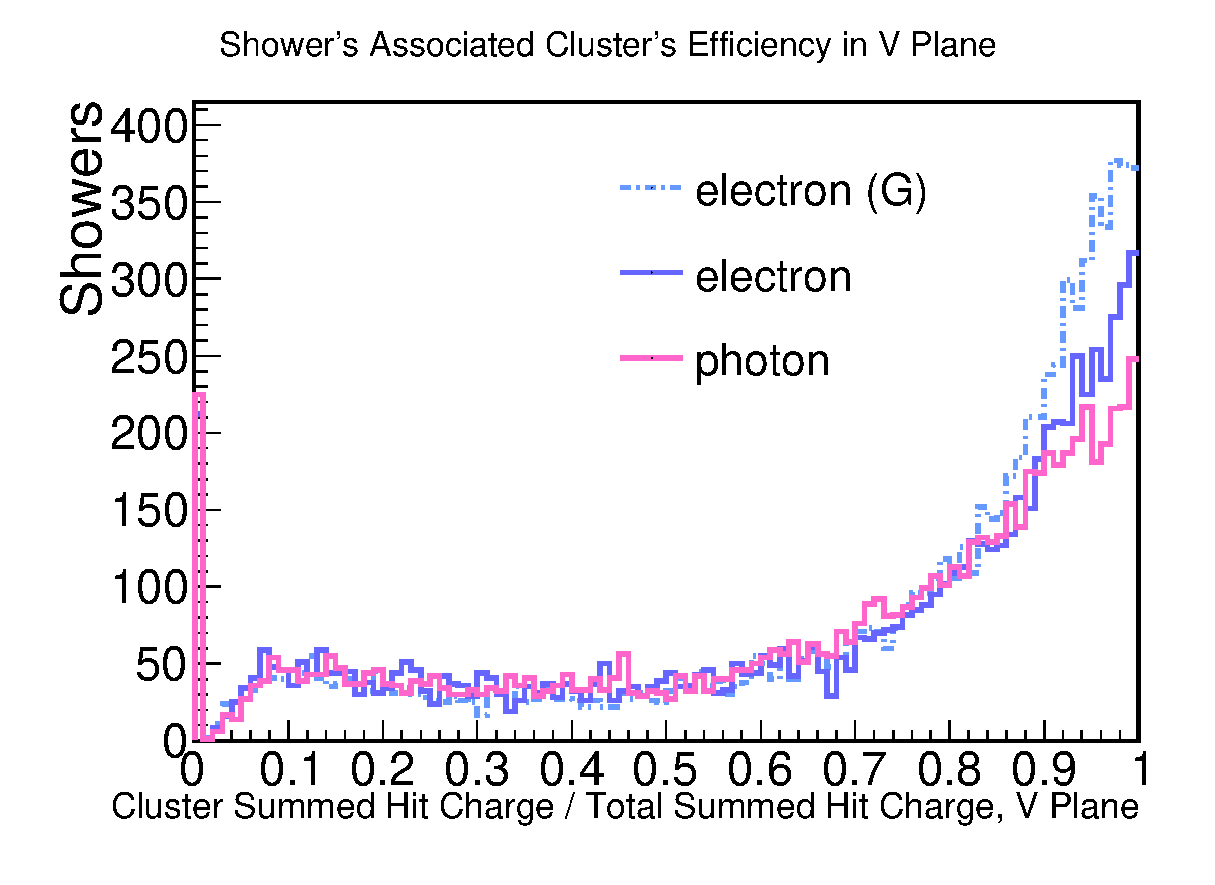
\includegraphics[width=0.3\textwidth]{figs/mc/single_em/ClusterEffV.eps}
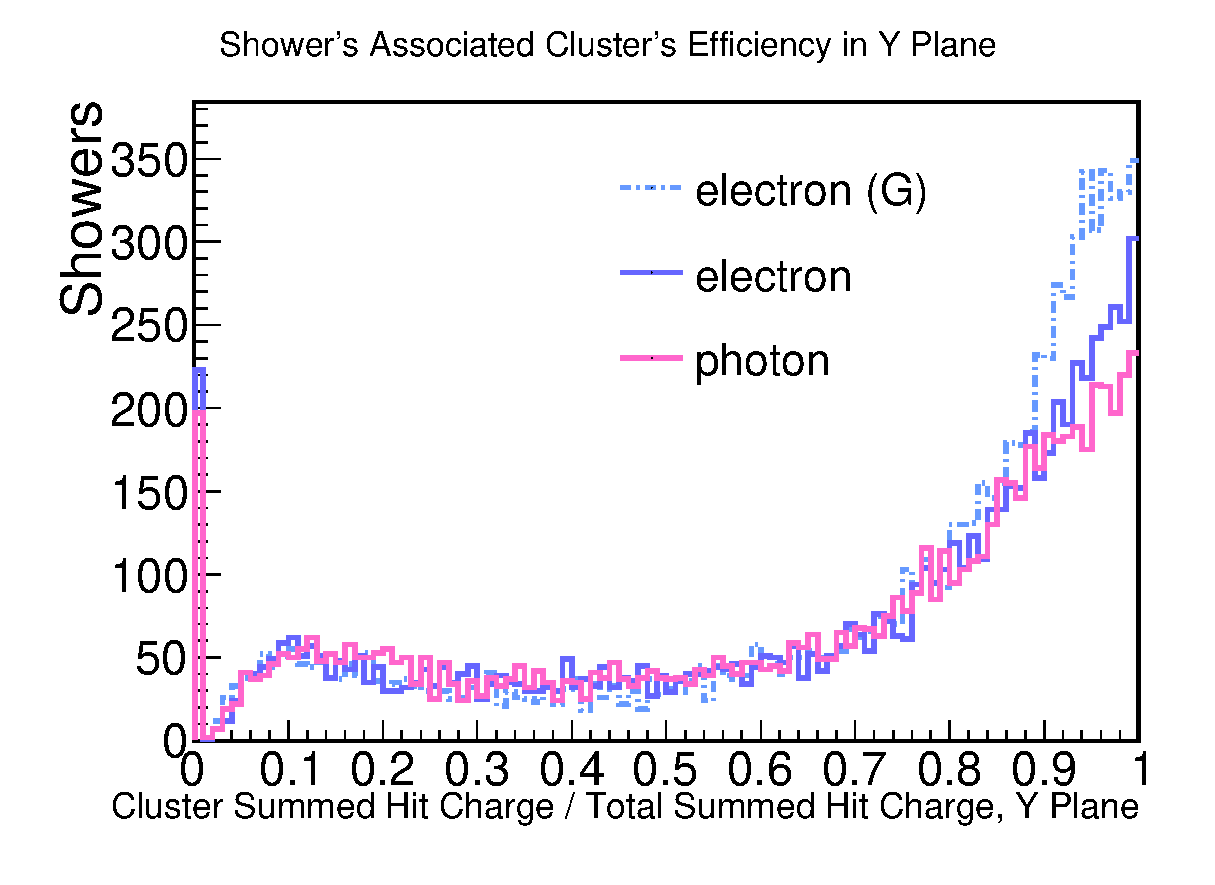
\includegraphics[width=0.3\textwidth]{figs/mc/single_em/ClusterEffY.eps}
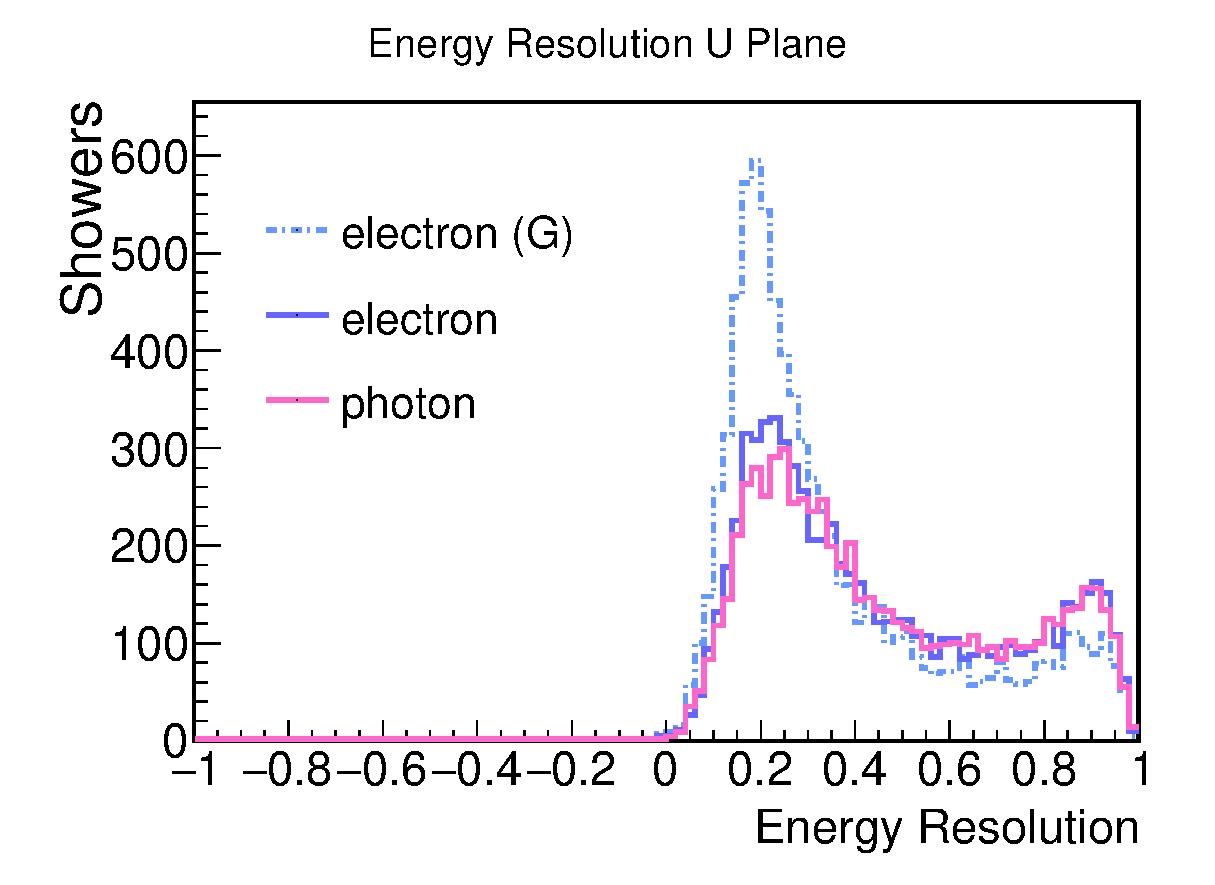
\includegraphics[width=0.3\textwidth]{figs/mc/single_em/EnergyResU.eps}
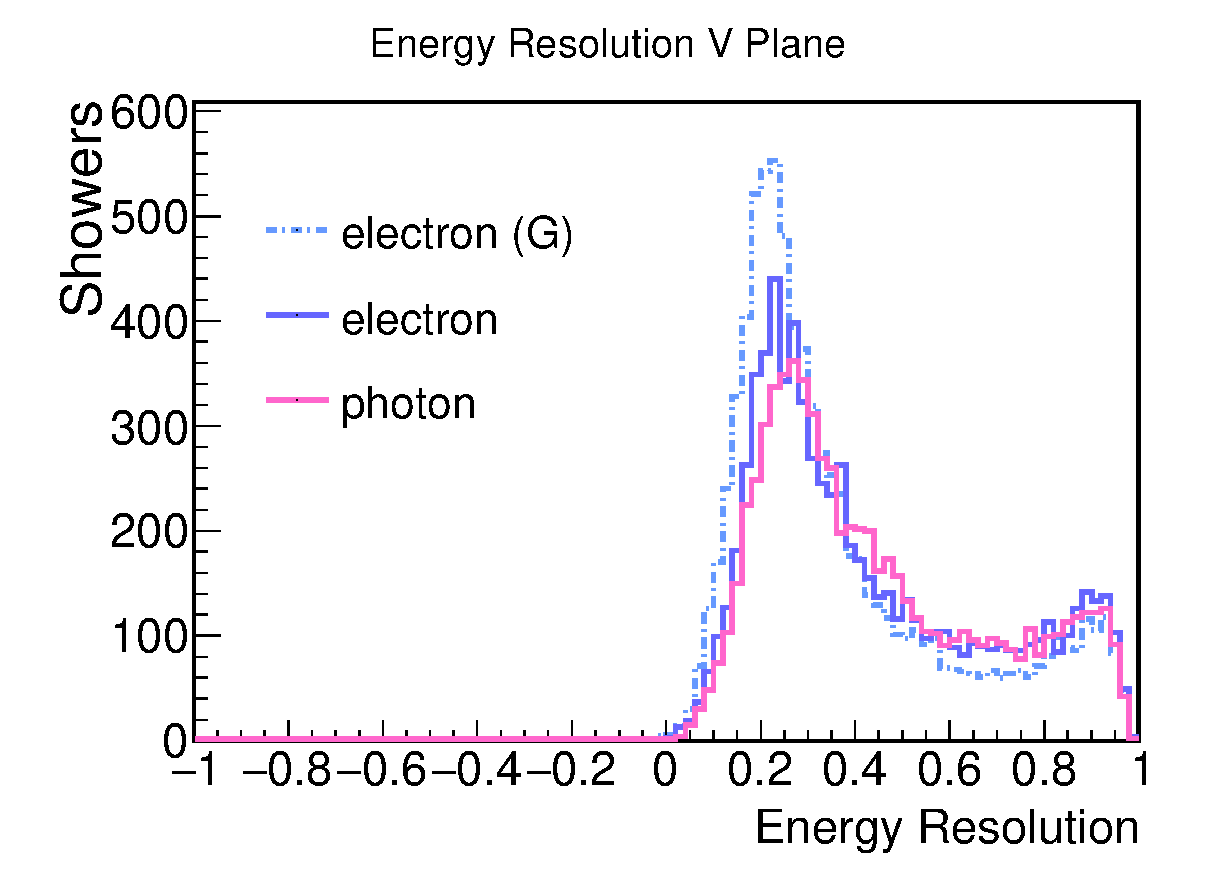
\includegraphics[width=0.3\textwidth]{figs/mc/single_em/EnergyResV.eps}
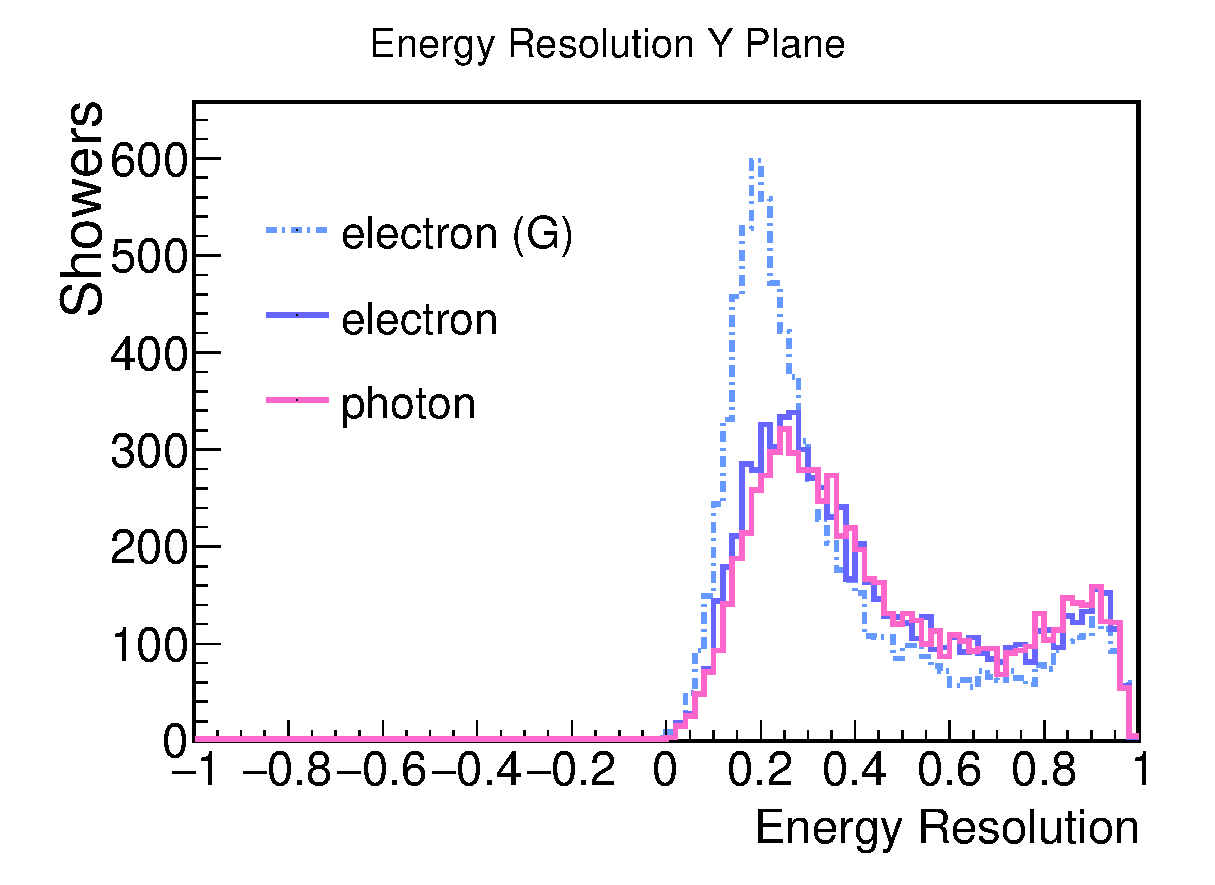
\includegraphics[width=0.3\textwidth]{figs/mc/single_em/EnergyResY.eps}
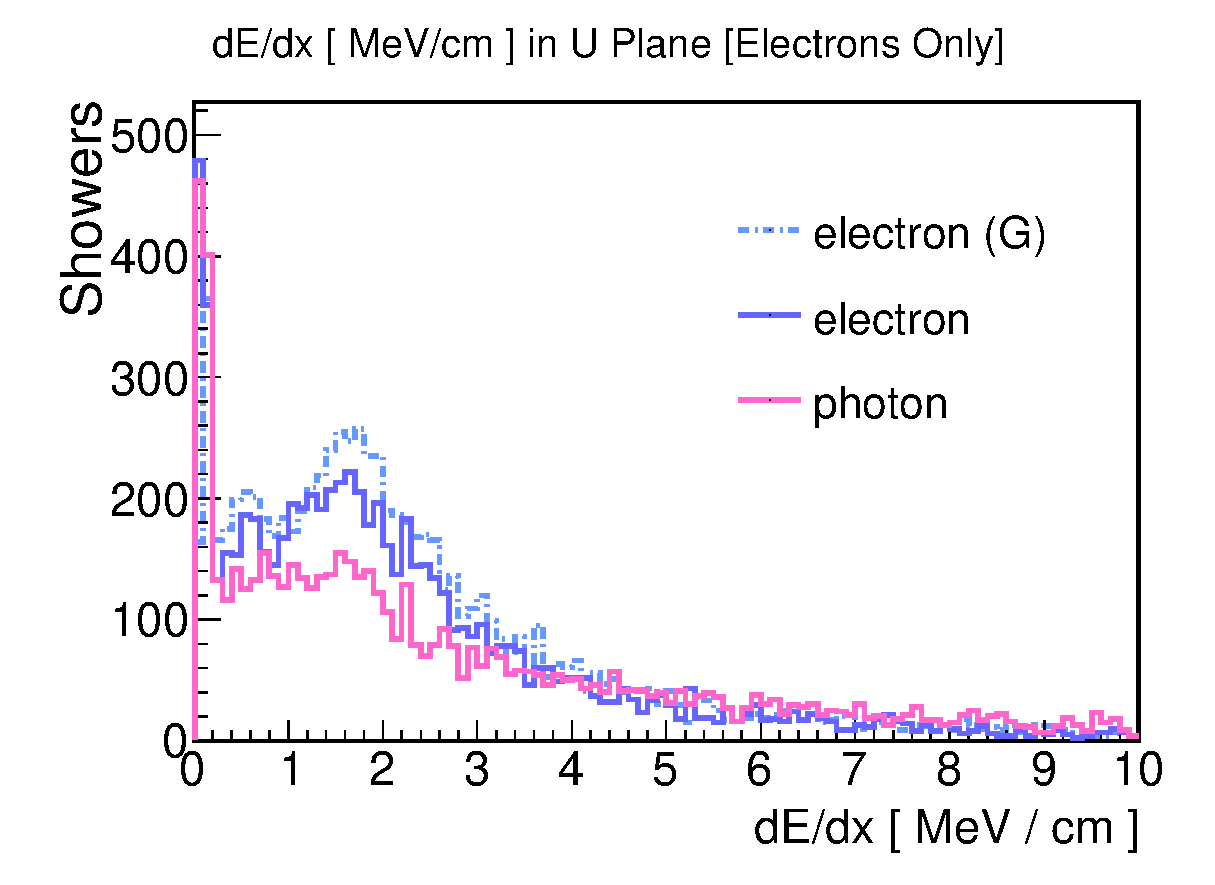
\includegraphics[width=0.3\textwidth]{figs/mc/single_em/dEdxU.eps}
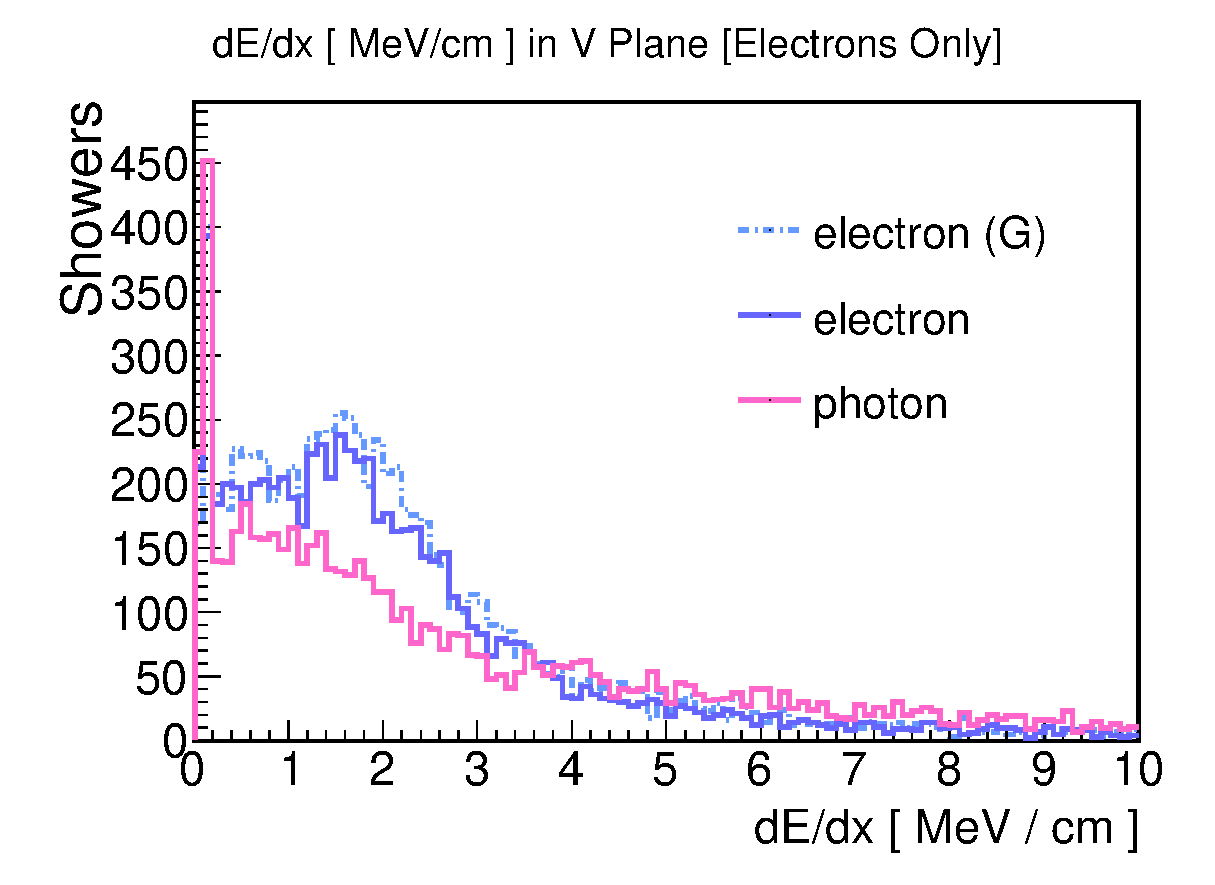
\includegraphics[width=0.3\textwidth]{figs/mc/single_em/dEdxV.eps}
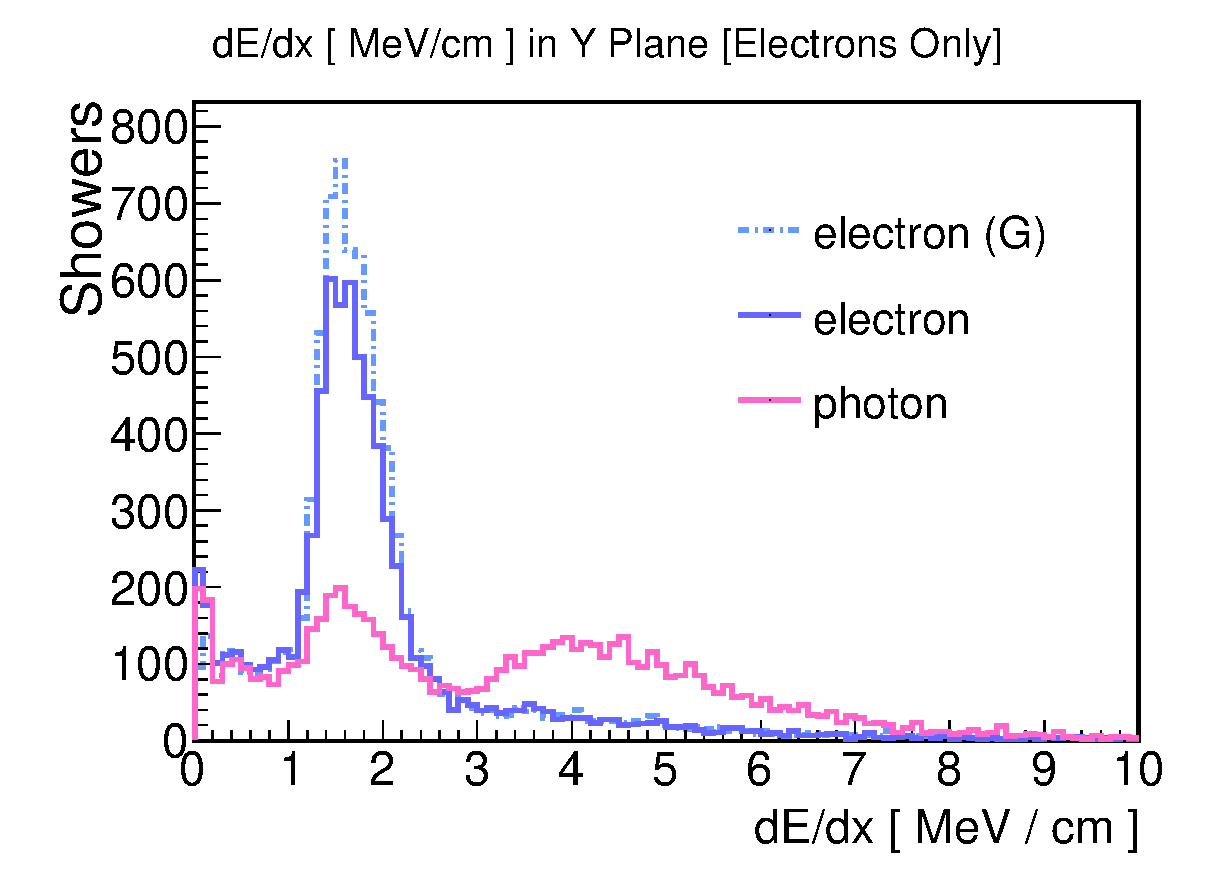
\includegraphics[width=0.3\textwidth]{figs/mc/single_em/dEdxY.eps}
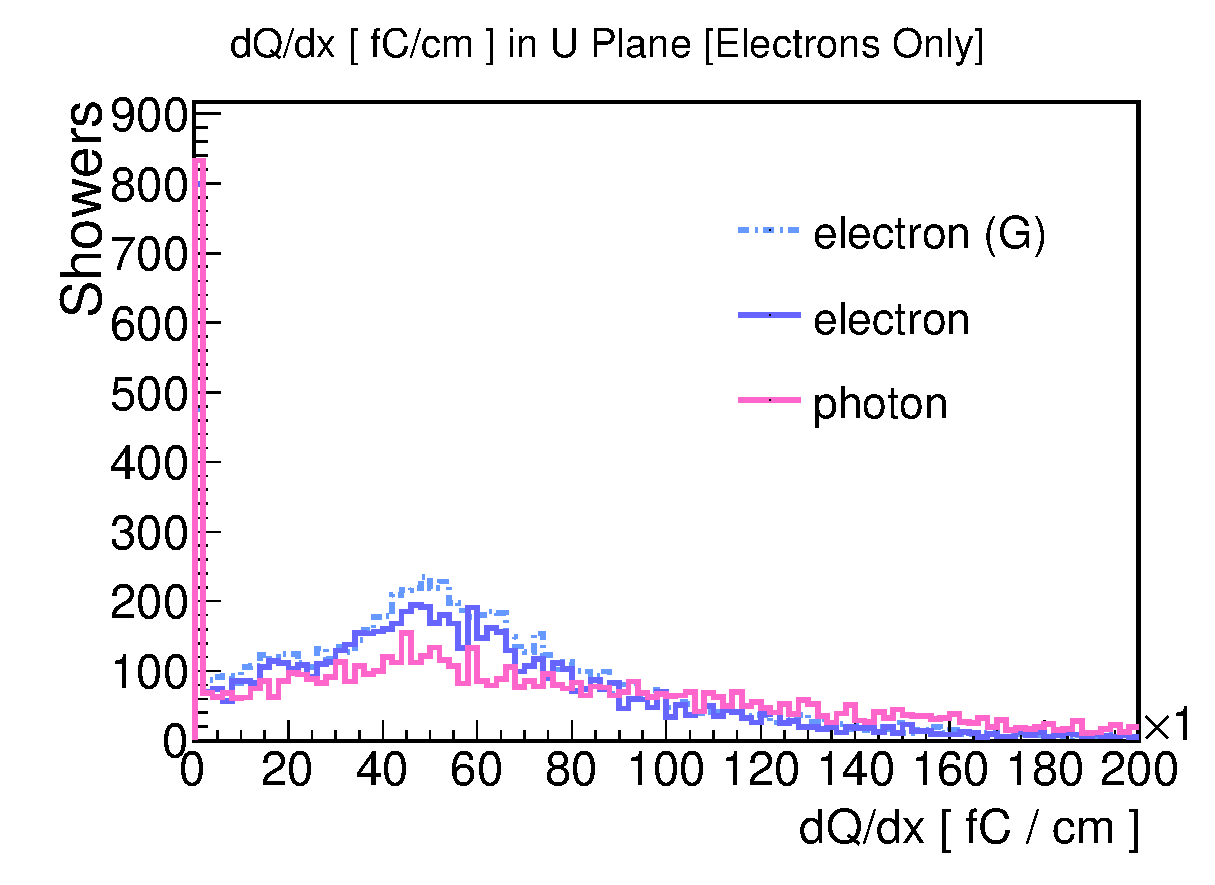
\includegraphics[width=0.3\textwidth]{figs/mc/single_em/dQdxU.eps}
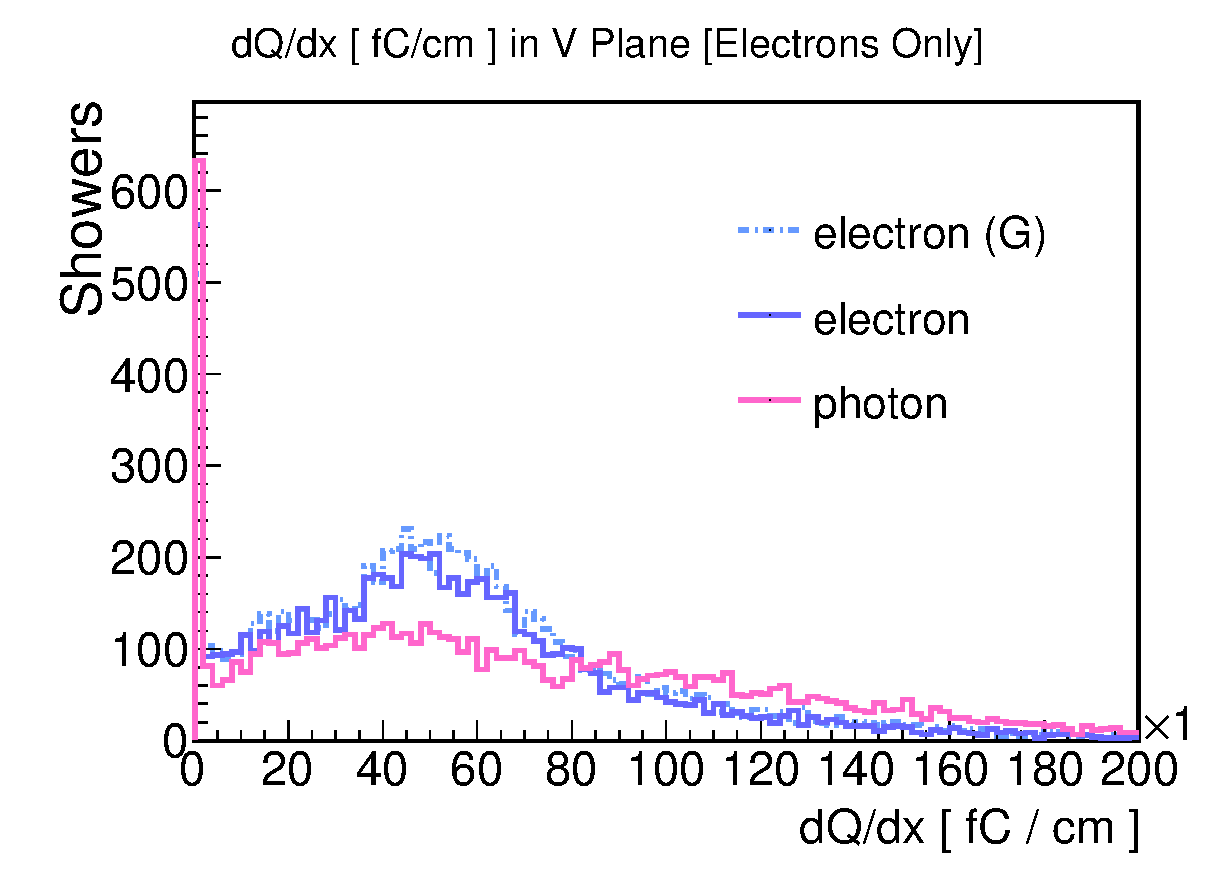
\includegraphics[width=0.3\textwidth]{figs/mc/single_em/dQdxV.eps}
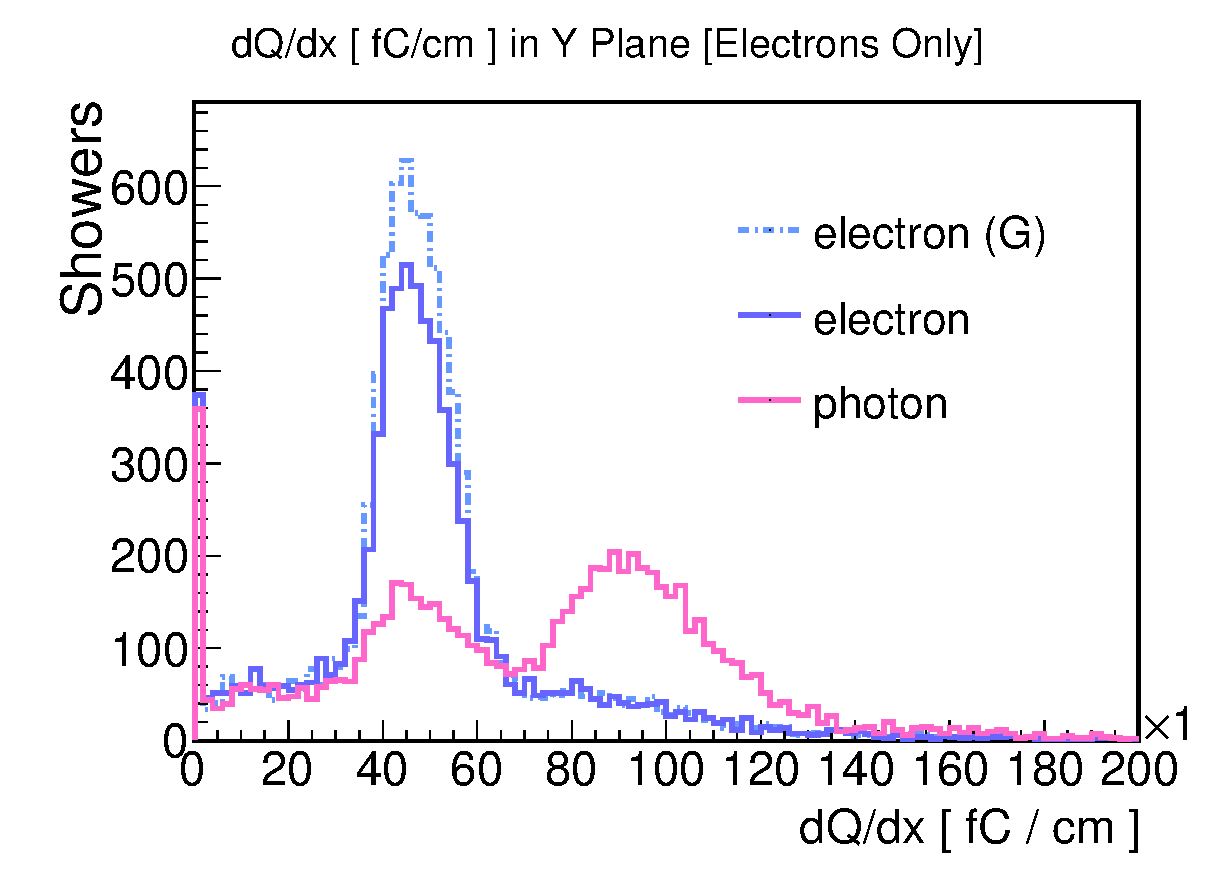
\includegraphics[width=0.3\textwidth]{figs/mc/single_em/dQdxY.eps}
\caption{Shower reconstruction quality of single electron and single
photon MC samples.  The legend (G) indicates the sample with the configuration
of all good wires.}
\label{fig:shr_quality_single_em}
\end{center}
\end{figure}
% --------------------------------------------------------------------


Energy deficiency is manifested in~\Cref{fig:shr_quality_single_em}.
Possible sources may come from
\begin{itemize}
\item charge deposits below the threshold of the hit finder,
\item missing charge deposits owing to bad wires,
\item clustering inefficiency,
\item energy calibration.
\end{itemize}
We further discuss the sources in~\Cref{sec:ongoing}. 
The peaks at zero in all the clustering efficiency and calorimetry
plots illustrate the feature of Pandora that it is not necessary to
have information in all the three wire planes to reconstruct a 
PFParticle.


% -----------------------------------------------------------------------
\clearpage
\subsection{Single $\pi^0$ Sample}
\label{sec:single_pi0}

Reconstruction of the $\pi^0$ invariant mass is a benchmark of
shower reconstruction qualities, as both the energy and
direction are involved,
\begin{equation}
\label{eq:pi0_mass}
m_{\pi^0} = \sqrt{2E_1 E_2(1-\cos\theta_{12})},
\end{equation}
where $E_1$ and $E_2$ represent the energy of the two photons
from the $\pi^0$ decay, and $\theta_{12}$ the angle between the
two photons.\\
\\
To examine the reconstruction of $\pi^0$ mass, 10,000 single $\pizero$
Monte Carlo events are generated with the momentum and
angular distributions identical to those in the single electron
and photon samples detailed in~\Cref{sec:single_em}.
Moreover, the simulation and reconstruction configuration is
exactly the same as that in the other samples; for instance,
the shower reconstruction is performed on shower-like PFParticles
in the plots illustrated here.\\
\\
The reconstructed showers are matched to the MC showers according
to the timing and the waveforms on the wires.
We select the events with the following criteria,
\begin{itemize}
\item containing exactly two reconstructed and matched showers,
\item both reconstructed energy greater than 0.1~MeV,
\item recontructed $\cos\theta_{12}$ less than 1,
\end{itemize}
and the $\pizero$ mass obtained from those two showers
are shown in~\Cref{fig:mpi0_single_pi0}.
In other words, the $\pizero$ mass is reconstructed from the perfect
combination of reconstructed showers.
1,816 events fulfill these criteria out of 10,000 single $\pizero$s,
and a resonance peak is presented in the $\pizero$ mass distribution.
Owing to the energy deficiency discussed in 
both~\Cref{sec:single_em,sec:ongoing}, the peak is not centered at
135~MeV.
Along with this issue, a study significantly improving the efficiency 
is discussed in~\Cref{sec:merging}.\\
\\
% --------------------------------------------------------------------
% Figure: pi0 mass
\begin{figure}[htbp]
\begin{center}
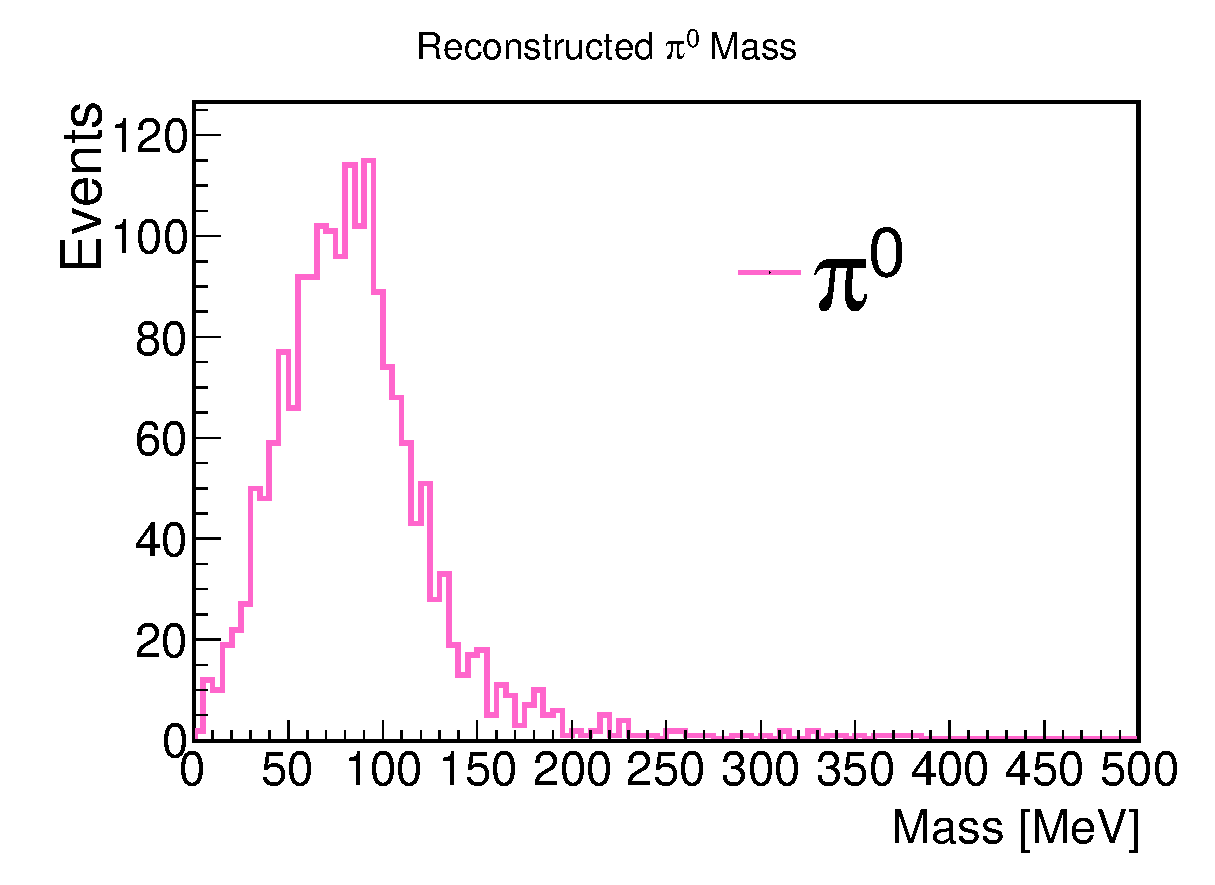
\includegraphics[width=0.75\textwidth]{figs/mc/single_pi0/RecoPi0Mass.eps}
\caption{Reconstructed $\pizero$ mass distribution from the single $\pizero$
MC sample.}
\label{fig:mpi0_single_pi0}
\end{center}
\end{figure}
% --------------------------------------------------------------------
% DCA, MC/reco combination to check the features of the pi0 mass 
% distributions
We further investigate the distance of closest approach between
the $\pizero$ decay point from the MC truth information and
the reconstructed shower direction.
\Cref{fig:dca_single_pi0} presents the distance of the closest
approach between the two reconstructed shower axes and the
true $\pizero$ decay point,
demonstrating the reconstructed shower direction is reasonable.
In addition, as shown in~\Cref{fig:mc_reco_single_pi0},
we check the impact of the energy and direction by
combining quatities from MC showers
and reconstructed showers,
\begin{itemize}
\item MC truth energy and direction: a $\delta$-function at 135~MeV,
\item MC deposited energy and MC truth direction: the long tail
      represents the energy outside the detector,
\item MC deposited energy and reconstructed direction: the smeared
      direction results in the long tail in the $\pizero$ mass distribution,
\item reconstructed energy and MC truth direction: the deficit in
      the reconstructed energy results in the position of the peak,
      as well as the width of the distribution.
\end{itemize}

% --------------------------------------------------------------------
% Figure: DCA
\begin{figure}[htbp]
\begin{center}
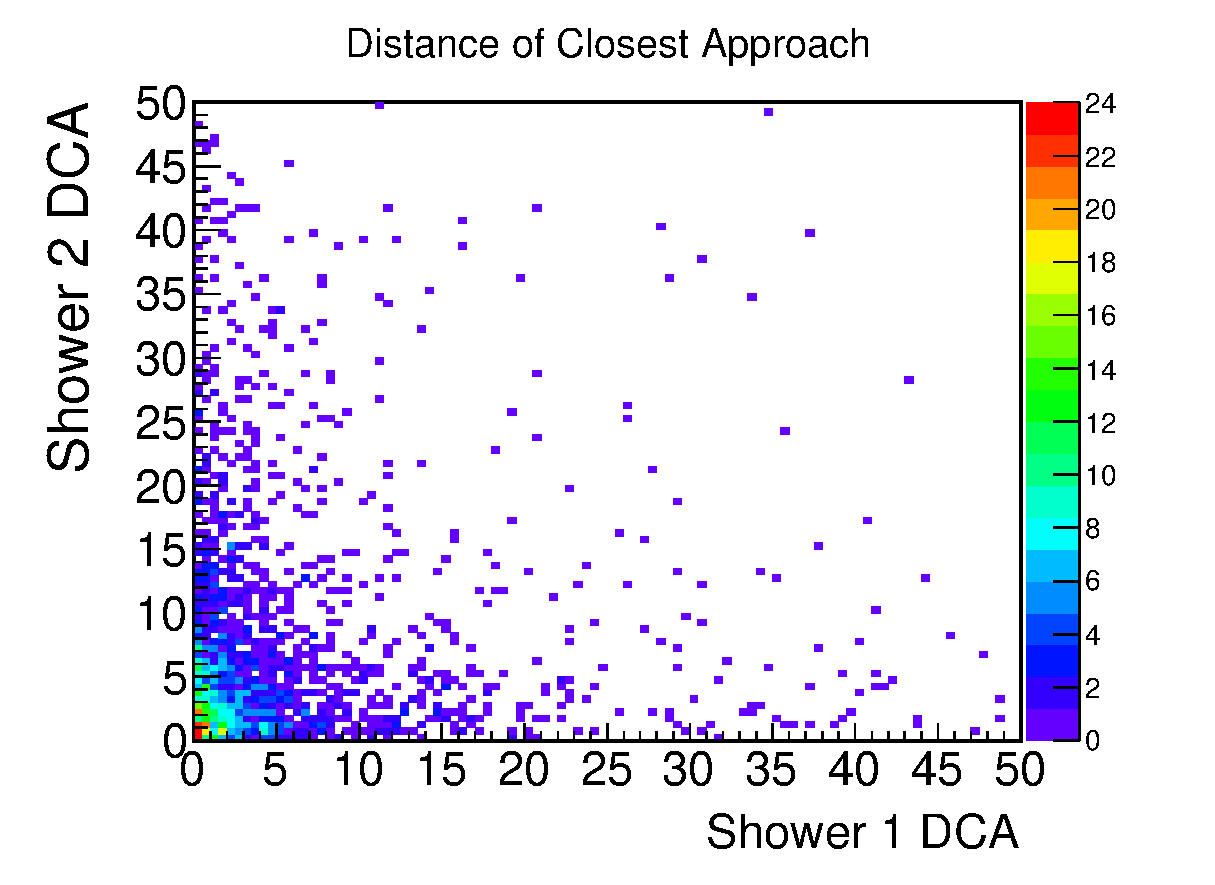
\includegraphics[width=0.75\textwidth]{figs/mc/single_pi0/pi0_DCA.eps}
\caption{The distance of closest approach from the two reconstructed
shower axes to the true $\pizero$ decay points.}
\label{fig:dca_single_pi0}
\end{center}
\end{figure}
% --------------------------------------------------------------------
% --------------------------------------------------------------------
% Figure: MC+Reco
\begin{figure}[htbp]
\begin{center}
\begin{subfigure}{0.45\textwidth}
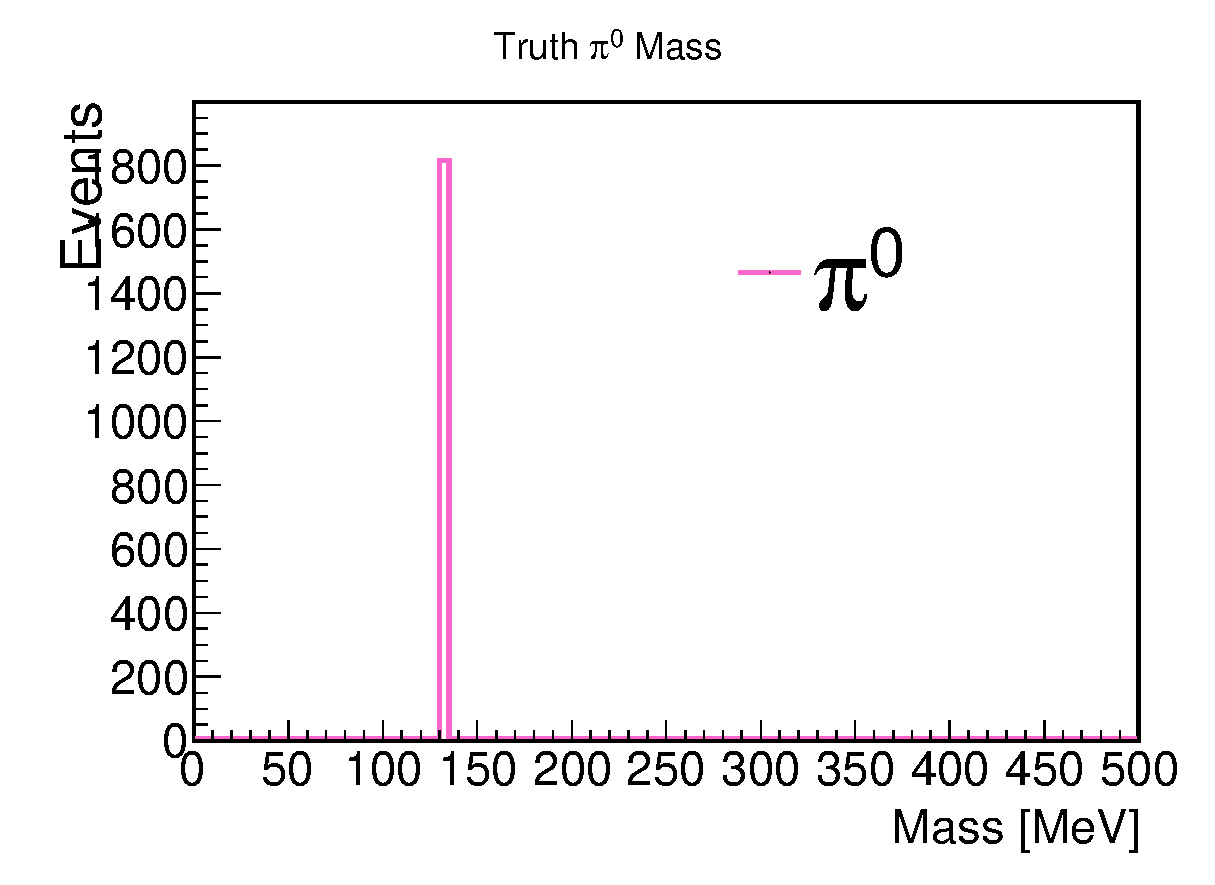
\includegraphics[width=0.9\linewidth]{figs/mc/single_pi0/MCPi0Mass.eps}
\caption{}
\end{subfigure}
\begin{subfigure}{0.45\textwidth}
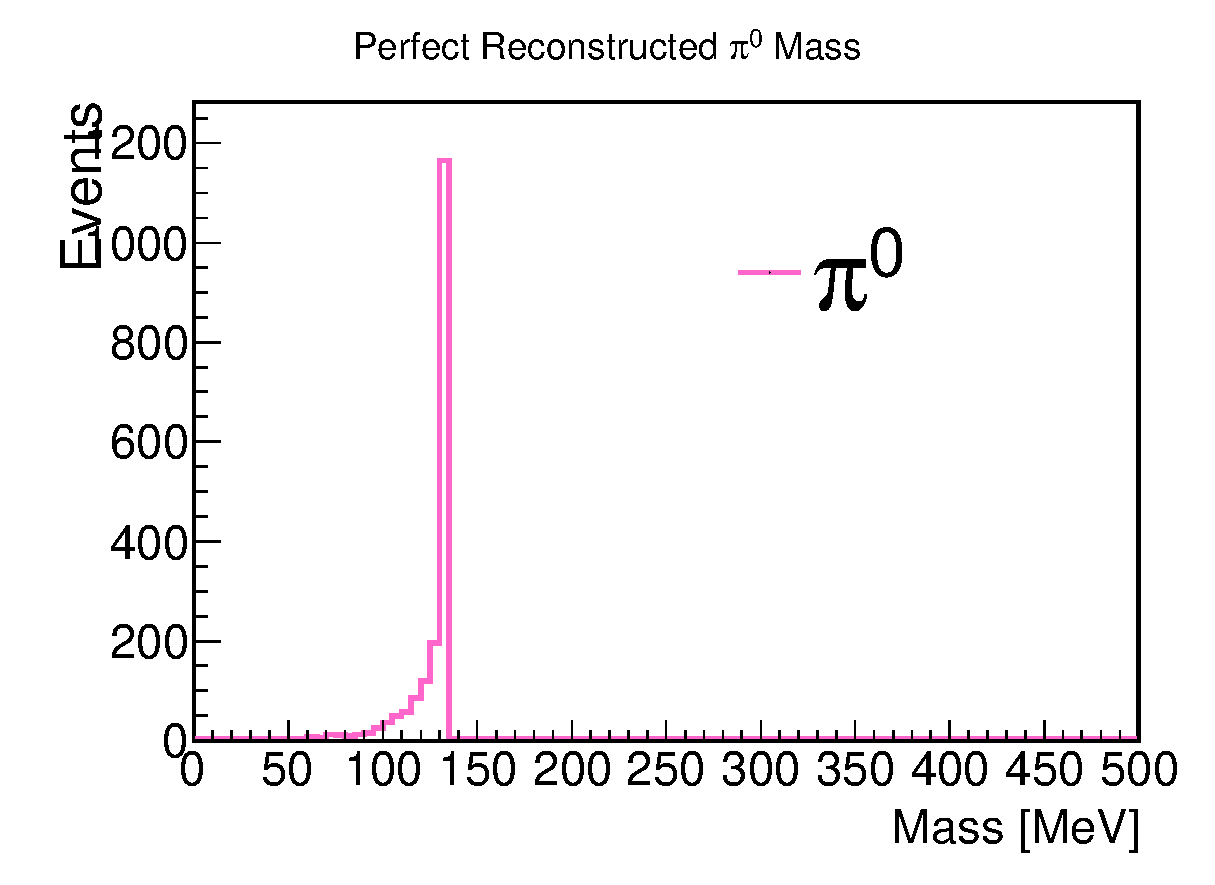
\includegraphics[width=0.9\linewidth]{figs/mc/single_pi0/PerfectRecoPi0Mass.eps}
\caption{}
\end{subfigure}
\begin{subfigure}{0.45\textwidth}
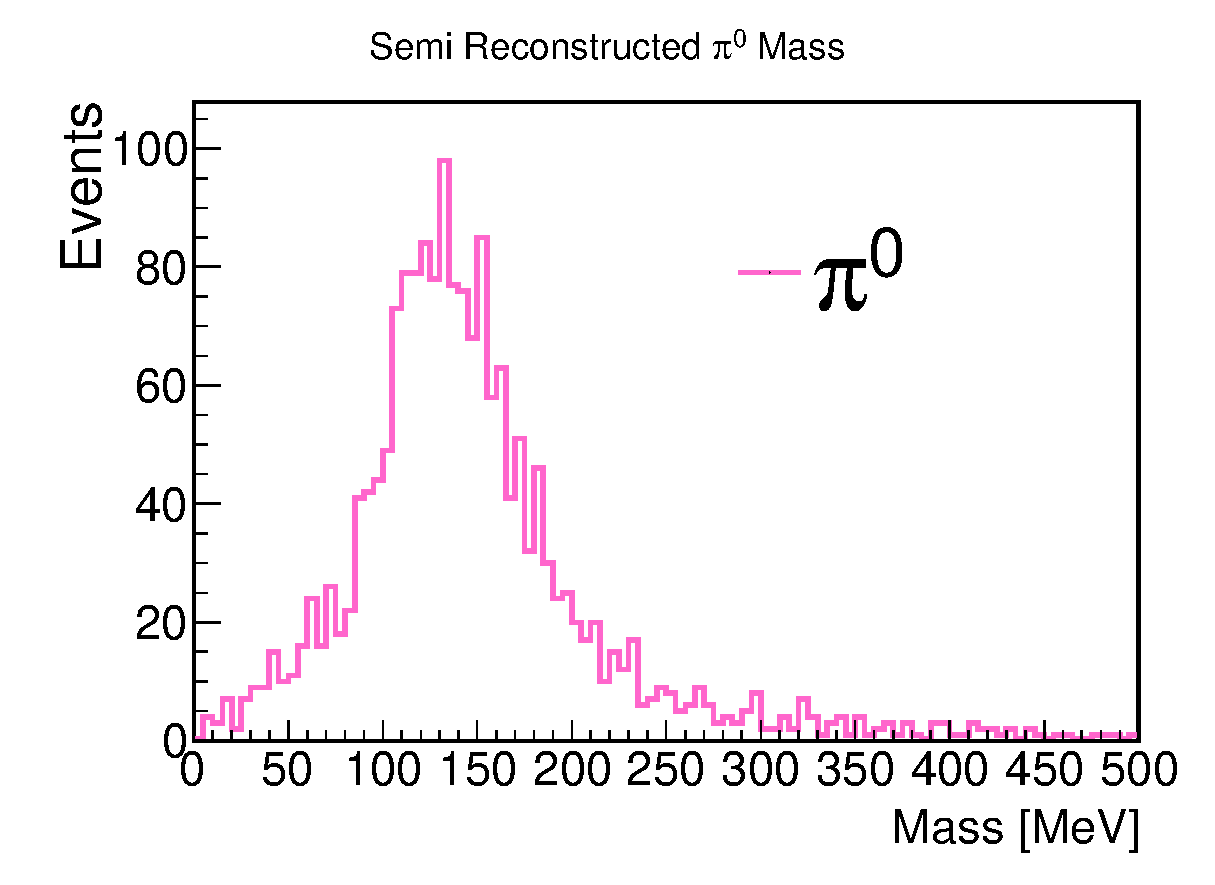
\includegraphics[width=0.9\linewidth]{figs/mc/single_pi0/DepERecoThetaPi0Mass.eps}
\caption{}
\end{subfigure}
\begin{subfigure}{0.45\textwidth}
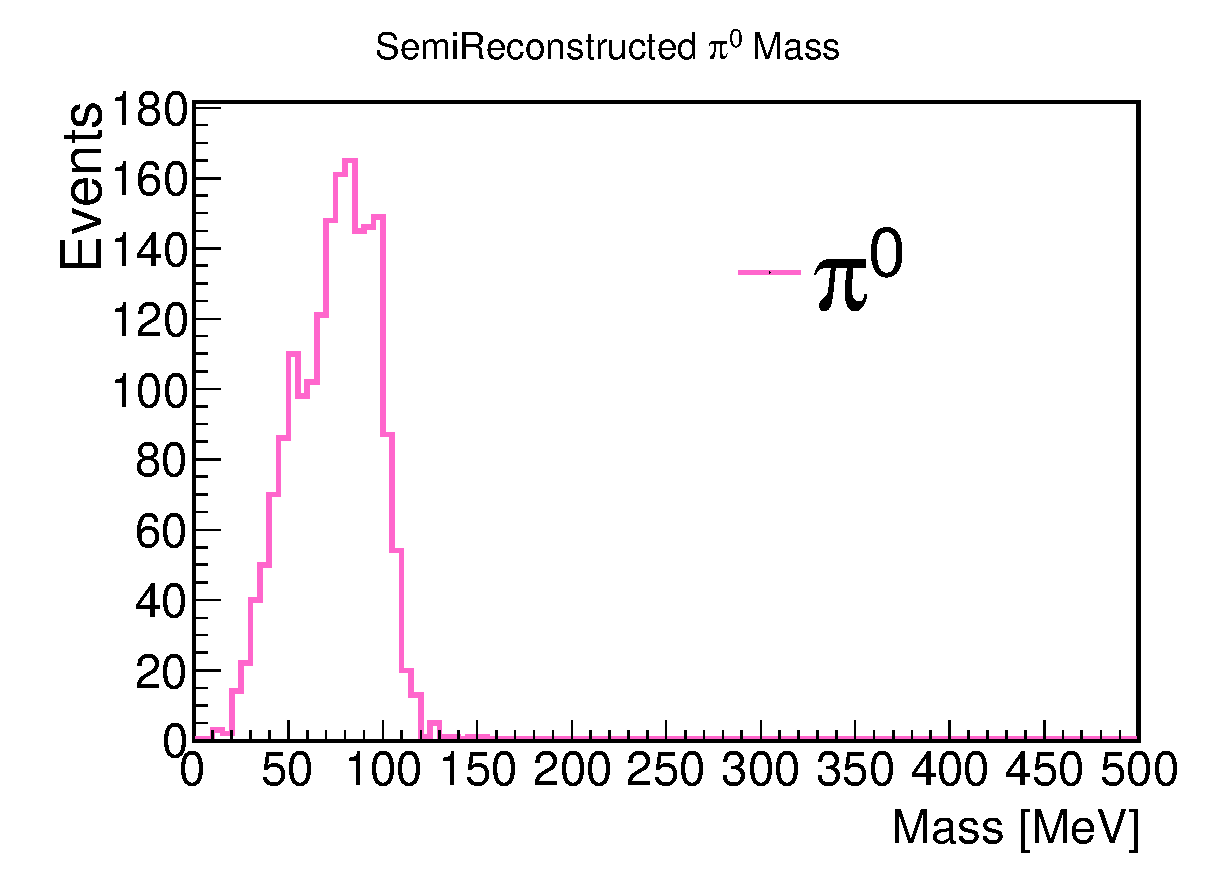
\includegraphics[width=0.9\linewidth]{figs/mc/single_pi0/RecoEMCThetaPi0Mass.eps}
\caption{}
\end{subfigure}
\caption{$\pizero$ mass distribution from (a) true energy and true direction,
(b) true deposited energy and true direction, (c) true deposited energy
and reconstructed direction, and (d) reconstructed energy and true direction.}
\label{fig:mc_reco_single_pi0}
\end{center}
\end{figure}
% --------------------------------------------------------------------
% -----------------------------------------------------------------------
\subsection{Full BNB Neutrinos and Cosmic Sample}
\label{sec:bnb}

We have not started studies on the simulated BNB neutrino samples,
but plan to do so.




% pi0 Reconstruction in data
\section{$\pi^{0}$ Mass Reconstruction in Data}


% Data
% \section{Data}


% Summary
\section{Summary}
\label{sec:summary}

In summary, we describe the automated shower reconstruction based 
on the outputs of Pandora pattern recognition,
and the subsequent $\pizero$ mass reconstruction.
We study single electron, photon, and $\pizero$ Monte Carlo
simulation, and apply the algorithms to a set of six data events
which are identified as charged current $\pizero$ production
by the $\nu_{\mu}$ charged current inclusive filter,
\texttt{PiZeroROI} selection, and handscanning.
% The particle flow clustering and 
% shower reconstruction used in 
% this note are fully automated.
Five of these data events have two showers with nonzero energy
from a neutrino candidate, and the reconstructed mass is
\begin{equation}
\label{eq:pi0_mass_result}
m_{\pizero} = 106.76\pm 12.84~\mbox{MeV (stat.)}
\end{equation}
The statistics are too low to draw a conclusion.


%---------------------------------------------------------------------

% \bibliographystyle{aiaa}
% \bibliographystyle{apacite}
% \bibliographystyle{alpha}
% \bibliography{tex/thesis}

%---------------------------------------------------------------------


\end{document}  
